
%\begin{lead}
%種々の信号処理は,信号処理システムにより実現される.そこで,ここでは離散時間信号を処理するシステムの考え方を導入する.ここで説明するシステムは,線形時不変システムと呼ばれるもので,非常に多く応用されている.信号値の乗算,加減算,信号値を記憶して時間シフト,の3種類の処理の組合せとして,ハードウェア,ソフトウェアのどちらでも実現可能である.

%\end{lead}

%\vfill

%\begin{koumoku}
%信号処理システム\\
%線形時不変システム\\
%3点平均\\
%\end{koumoku}


%\chapter{信号処理システム}
%\label{chapter:ch-2}



\section*{章末問題の略解}
\addtocontents{toc}{\onelineskip}\addcontentsline{toc}{section}{章末問題の略解}
\stepcounter{chapter}
\subsection*{第\ref{chapter:intro}章}

\subsubsection*{問題\ref{chapter:intro}.1}

画像の幾何学的形状の変形は,座標系に拡大・縮小・回転を加えることで実現可能である.たとえば眼だけ大きく見せるためには,眼の中心部分に原点をおき,眼が存在する領域だけ拡大できるように座標系を置き換えればよい.

\subsubsection*{問題\ref{chapter:intro}.2}

画像の尖鋭化を行う場合,輪郭となる部分が強調されるという長所があるとともに,ごま塩雑音などのような雑音も強調されるという短所がある.

画像のぼかしを行う場合,ごま塩雑音などのような雑音が低減されるという長所があるとともに,輪郭となる部分がぼけてしまうという短所がある.

\subsubsection*{問題\ref{chapter:intro}.3}

人間の可聴音は20Hz~20kHzであるとされている.その上限である20kHzの2倍以上である44.1kHzであれば,サンプリング定理により20kHzの音声信号を復元可能とされるためである.

\subsection*{第\ref{chapter:2}章}

\subsubsection*{問題\ref{chapter:2}.1}

\noindent (1) $A=1$,$\theta=\displaystyle \frac{-\pi}{3}$,
(2) $A=\sqrt{(1+\displaystyle \cos \frac{-\pi}{3})^2+\sin^2 \theta}=\displaystyle \frac{\sqrt{15}}{2}$,$\theta=\tan^{-1}\displaystyle \frac{2}{3}$,\\
(3) $A=\displaystyle \frac{\sqrt{(x^2-9)^2 + 36x^2}}{x^2+9}$,$\theta=\displaystyle \frac{6x}{(x^2-9)}$,
(4) $A=\displaystyle \sqrt{ R^2+ \left( \omega L - \frac{1}{\omega C} \right)^2}$,$\theta=\displaystyle \frac{\omega^2 LC -1}{\omega CR}$

\subsubsection*{問題\ref{chapter:2}.2}

\noindent (1) $\theta=\displaystyle \frac{\pi}{3}$, $\pi$,
\noindent (2) $\displaystyle \frac{-5}{18}$

\subsubsection*{問題\ref{chapter:2}.3}

\noindent (1) 0,(2) $\displaystyle \frac{1}{4}$,(3) 0 ($y=1/x$とおいて解くとよい),(4) 0

\subsubsection*{問題\ref{chapter:2}.4}

\noindent (1) $2x$,(2) $\displaystyle \frac{-3x^2+2x-15}{(x^2-5)^2}$,(3) $\displaystyle \frac{4t}{(t^2+1)^2}$,(4)$\displaystyle -\frac{3}{2x^3\sqrt{x}}$,(5) $-3\cos (2-3x)$,\\
(6) $\displaystyle \frac{1}{\cos^2(x-2)}$,(7) $2e^{2x+5}$,(8) $e^{3x}(3\cos (2x+1)-2\sin (2x+1))$,\\
(9) $\displaystyle \frac{5^x}{\log_e 5}$ (両辺の対数をとり,陰関数の微分による)

\subsubsection*{問題\ref{chapter:2}.5}

ここでは$C$を積分定数とする.

\noindent (1) $\displaystyle \frac{1}{2}x^4+x^3-2x^2+5x+C$, (2) $\displaystyle \frac{3}{4}\sqrt[3]{(2x+3)^2}+$, (3) $\displaystyle \frac{1}{2} \sin (4x+1) +\frac{1}{2} \cos 2x + C$,
\\
(4) $\displaystyle e^x - \frac{1}{3}e^{-3x}+C$,(5) $\displaystyle \frac{1}{2} \tan 2x -x+C$,
(6) $\displaystyle \frac{a}{a^2+b^2}e^{ax}\sin bx -\frac{b}{a^2+b^2}e^{ax}\cos bx +C$

\subsubsection*{問題\ref{chapter:2}.6}

\noindent (1) $\displaystyle -\frac{20}{3}$, (2) $\displaystyle \frac{14}{3}+2\log 2$,
(3) $\displaystyle 1-\frac{\sqrt{3}}{4}$, (4) 0, 
(5) $\displaystyle \frac{\pi}{6}$, (6) $\displaystyle \frac{\pi}{6\sqrt{3}}$

\subsubsection*{問題\ref{chapter:2}.7}

\noindent (1) $\displaystyle \frac{1}{1-z^{-1}}$ ただし$|z^{-1}|<1$, (2) $\displaystyle \frac{3}{4}$ 

\subsubsection*{問題\ref{chapter:2}.8}

\noindent (1) $\displaystyle 1-\frac{x^2}{2!}+\frac{x^4}{4!}-\cdots$,(2) $\displaystyle x-\frac{x^3}{3!}+\frac{x^5}{5!}-\cdots$,(3) $\displaystyle x-\frac{x^2}{2}+\frac{x^3}{3}-\cdots$

\subsection*{第\ref{chapter:3}章}

\subsubsection*{問題\ref{chapter:3}.1}

以下の解図のようになる.

\begin{figure}[H]
\begin{center}

\begin{minipage}[b]{.32\textwidth}
\begin{center}
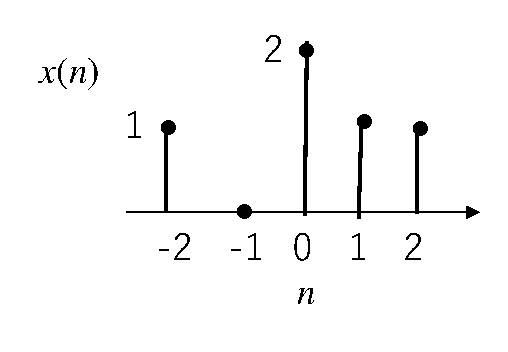
\includegraphics[height=2.8cm]{fig/zu-3e-1a.eps}

(1)
\end{center}
\end{minipage}
\begin{minipage}[b]{.25\textwidth}
\begin{center}
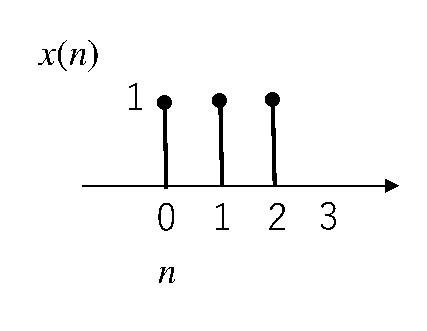
\includegraphics[height=2.6cm]{fig/zu-3e-1b.eps}

(2)
\end{center}
\end{minipage}
\begin{minipage}[b]{.35\textwidth}
\begin{center}
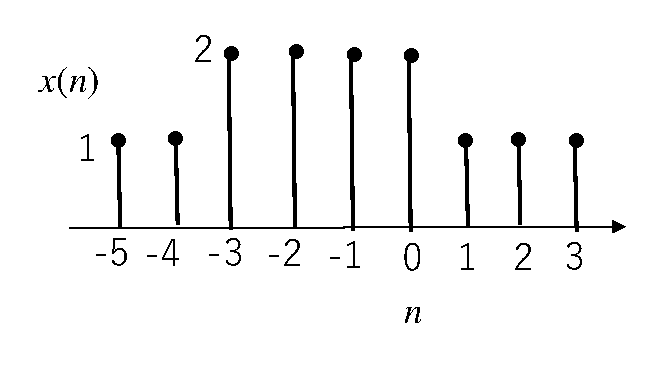
\includegraphics[height=2.5cm]{fig/zu-3e-1c.eps}

(3)
\end{center}
\end{minipage}

\end{center}
%\caption{問題\ref{chapter:3}.1の解図}
\end{figure}



\subsubsection*{問題\ref{chapter:3}.2}
\vskip-\baselineskip
\begin{displaymath}
T_s=\displaystyle \frac{1}{F_s}=2.27 \times 10^{-5}\textrm{sec} \nonumber
\end{displaymath}

このサンプリング周波数である44.1kHzはオーディオにおいて広く用いられるものである.

\subsubsection*{問題\ref{chapter:3}.3}

実際に取り扱うアナログ信号には雑音をはじめとした周波数帯の異なる成分が多く含まれることから,処理のために必要な成分を抽出するために,アナログフィルタを用いる.

\subsection*{第\ref{chapter:ch-2}章}

\subsubsection*{問題\ref{chapter:ch-2}.1}

\begin{enumerate}[(1)]
\item 線形性を満たさない.時普遍性を満たす.

\item 線形性を満たす.時普遍性を満たさない.

\item 線形性を満たす.時普遍性を満たさない.
\end{enumerate}

\subsubsection*{問題\ref{chapter:ch-2}.2}


以下に示す解図のようになる.

\begin{figure}[H]
\begin{center}

\begin{minipage}[b]{.3\textwidth}
\begin{center}
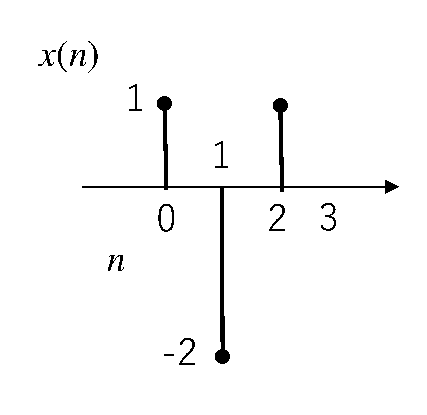
\includegraphics[width=.98\textwidth]{fig/zu-3e-2b.eps}

(1)
\end{center}
\end{minipage}
\begin{minipage}[b]{.3\textwidth}
\begin{center}
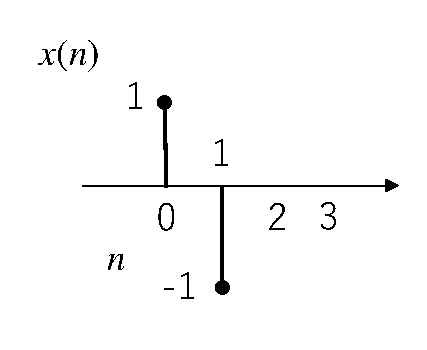
\includegraphics[width=.98\textwidth]{fig/zu-3e-2a.eps}

(2)
\end{center}
\end{minipage}
\begin{minipage}[b]{.3\textwidth}
\begin{center}
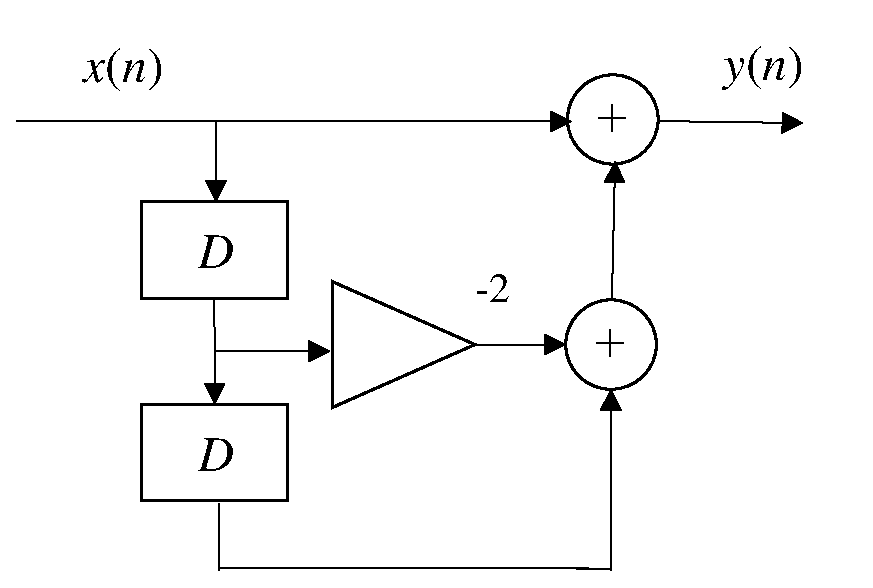
\includegraphics[width=.98\textwidth]{fig/zu-3e-2c.eps}

(3)
\end{center}
\end{minipage}

\end{center}
%\caption{問題\ref{chapter:ch-2}.2の解図}
\end{figure}

%問題\ref{chapter:ch-2}.3


%以下に示す解図のようになる.

%\begin{figure}[h]
%\begin{center}

%\begin{minipage}{4.5cm}
%\begin{center}
%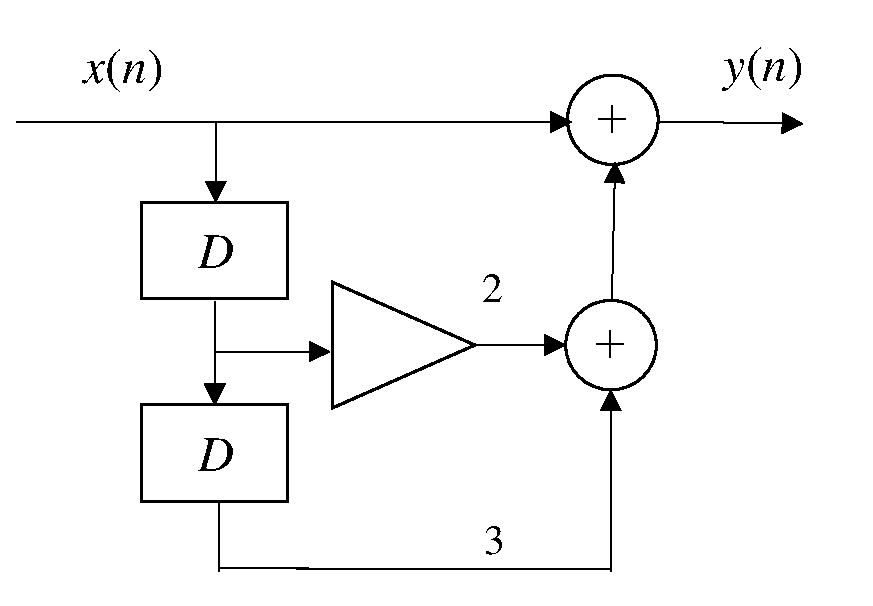
\includegraphics[width=4.5cm]{fig/zu-3e-3a.eps}

%(1)のハードウェア構成図
%\end{center}
%\end{minipage}
%\begin{minipage}{4.5cm}
%\begin{center}
%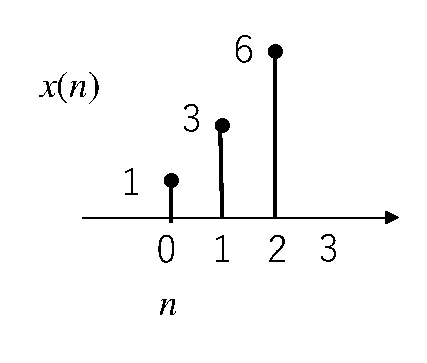
\includegraphics[width=3.5cm]{fig/zu-3e-3b.eps}

%(1)のインパルス応答
%\end{center}
%\end{minipage}

%\begin{minipage}{4.5cm}
%\begin{center}
%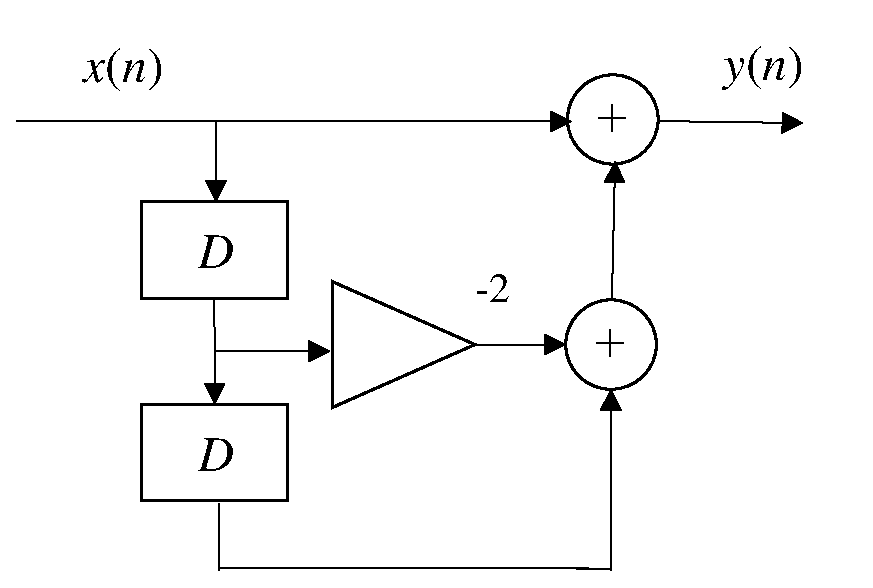
\includegraphics[width=4.5cm]{fig/zu-3e-2c.eps}

%(2)のハードウェア構成図
%\end{center}
%\end{minipage}
%\begin{minipage}{4.5cm}
%\begin{center}
%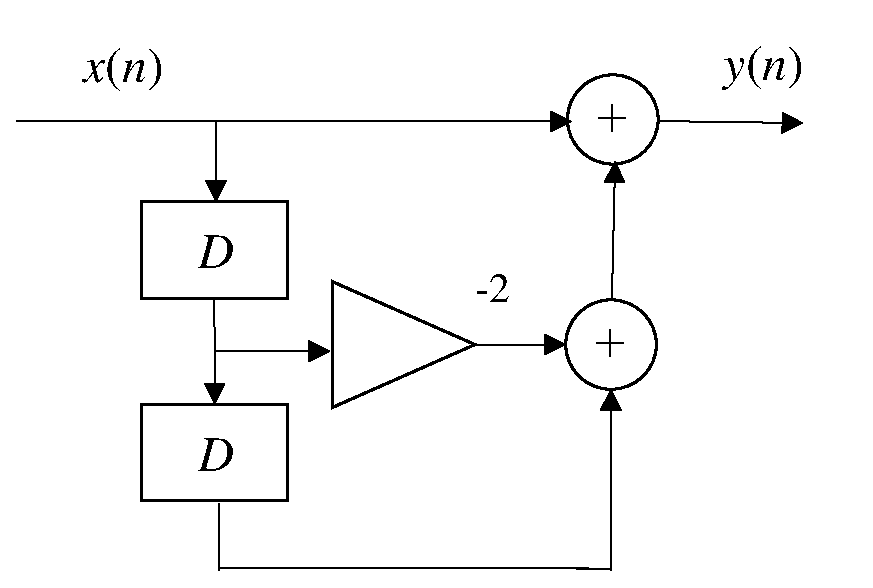
\includegraphics[width=4.5cm]{fig/zu-3e-2c.eps}

%(2)のインパルス応答
%\end{center}
%\end{minipage}

%\end{center}
%\caption{問題\ref{chapter:ch-2}.3の解図}
%\end{figure}


\subsection*{第\ref{chapter:40}章}

\subsubsection*{問題\ref{chapter:40}.1}
\vskip-\baselineskip
\begin{displaymath}
(1)  \hspace{3mm} X(z)=z^2+3-2z^{-1} 
\end{displaymath}
\begin{displaymath}
(2)  \hspace{3mm} X(z) = \frac{1}{1-z^{-1}} + \frac{2z^{-1}}{1-z^{-1}} = \frac{1+2z^{-1}}{1-z^{-1}} 
\end{displaymath}
\begin{displaymath}
(3) \hspace{3mm} X(z)= -b^{-1}z-b^{-2}z^2-b^{-3}z^3- \cdots =\frac{-b^{-1}z}{1-b^{-1}z} = \frac{1}{1-bz^{-1}} \nonumber
\end{displaymath}
\begin{displaymath}
(4) \hspace{3mm} x(n)= \frac{e^{j\omega n}-e^{-j\omega n}}{2j}u(n) \nonumber
\end{displaymath}
と書き換えることができるので\vskip.2\baselineskip
\begin{eqnarray}
X(z)&=&\frac{1}{2j(1-e^{j\omega}z^{-1})} - \frac{1}{2j(1-e^{-j\omega}z^{-1})}=\frac{(1-e^{-j\omega}z^{-1})-(1-e^{j\omega}z^{-1})}{2j(1-e^{-j\omega}z^{-1})(1-e^{j\omega}z^{-1})} \nonumber \\
&=&\frac{e^{j\omega}z^{-1}-e^{-j\omega}z^{-1}}{2j(1-(e^{j\omega}z^{-1}+e^{-j\omega}z^{-1})+z^{-2})}=\frac{\sin (\omega )z^{-1}}{1-2\cos (\omega )z^{-1}+z^{-2}} \nonumber 
\end{eqnarray}
\vskip.5\baselineskip
\subsubsection*{問題\ref{chapter:40}.2}
\vskip-\baselineskip
\begin{displaymath}
(1) \hspace{3mm} Y(z) =aX(z)+bX(z)z^{-d} \nonumber
\end{displaymath}
\begin{displaymath}
(2) \hspace{3mm} Y(z) = \sum_{n=-\infty }^{\infty }(-1)^nx(n)z^{-n} = \sum_{n=-\infty }^{\infty }x(n)(-z)^{-n} =X(-z) \nonumber
\end{displaymath}

\subsection*{第\ref{chapter:42}章}

\subsubsection*{問題\ref{chapter:42}.1}

\noindent (1) べき級数展開法を用いる.
\begin{displaymath}
x(n)=\delta (n+2)+ \delta(n) +2\delta(n-2) \nonumber
\end{displaymath}

\noindent (2) べき級数展開法を用い,$X(z)$を等比級数の和の表現とする.
\begin{displaymath}
X(z)=\sum_{n=0}^{\infty}(0.5z^{-1})^n \nonumber
\end{displaymath}
と書けるため
\begin{displaymath}
x(n)=0.5^nu(n) \nonumber
\end{displaymath}

\noindent (3) 部分分数分解法が既に用いられている.
\begin{displaymath}
x(n)=2(0.5)^nu(n-1)+u(n) \nonumber
\end{displaymath}

\noindent (4) 部分分数分解法を用いる.
\begin{displaymath}
X(z)=\frac{-1}{1-0.5z^{-1}}+\frac{2}{1-z^{-1}} \nonumber
\end{displaymath}
と書けるため
\begin{displaymath}
x(n)=-(0.5)^nu(n)+2u(n) \nonumber
\end{displaymath}

\subsubsection*{問題\ref{chapter:42}.2}
\vskip-\baselineskip
\begin{displaymath}
(1) \hspace{3mm} Y(z)=X(z)+aX(z)z^{-1}+bX(z)z^{-2}=(1+az^{-1}+bz^{-2})X(z) \nonumber 
\end{displaymath}
と書けることから,伝達関数$H(z)$は
\begin{displaymath}
H(z)=\frac{Y(z)}{X(z)}=1+az^{-1}+bz^{-2} \nonumber
\end{displaymath}
であるため,ハードウェア構成は下図のようになる.

%\begin{figure}[H]
\begin{center}
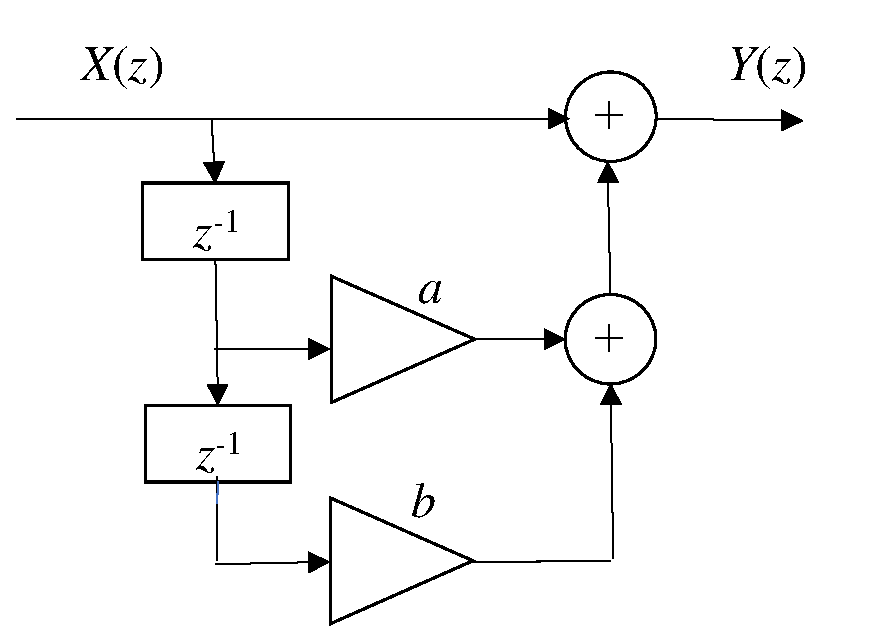
\includegraphics[width=6cm]{fig/zu-9e-1a.eps}
\end{center}
%\caption{システムのハードウェア構成}
%\label{fig:f-9e-a1}
%\end{figure}

\begin{displaymath}
(2) \hspace{3mm} Y(z)=X(z)+aX(z)z^{-1}+bY(z)z^{-2}=(1+az^{-1})X(z)+bz^{-2}Y(z) \nonumber 
\end{displaymath}
と書けることから,伝達関数$H(z)$は
\begin{displaymath}
H(z)=\frac{Y(z)}{X(z)}=\frac{1+az^{-1}}{1-bz^{-2}} \nonumber
\end{displaymath}
であるため,ハードウェア構成は下図のようになる.

%\begin{figure}[H]
\begin{center}
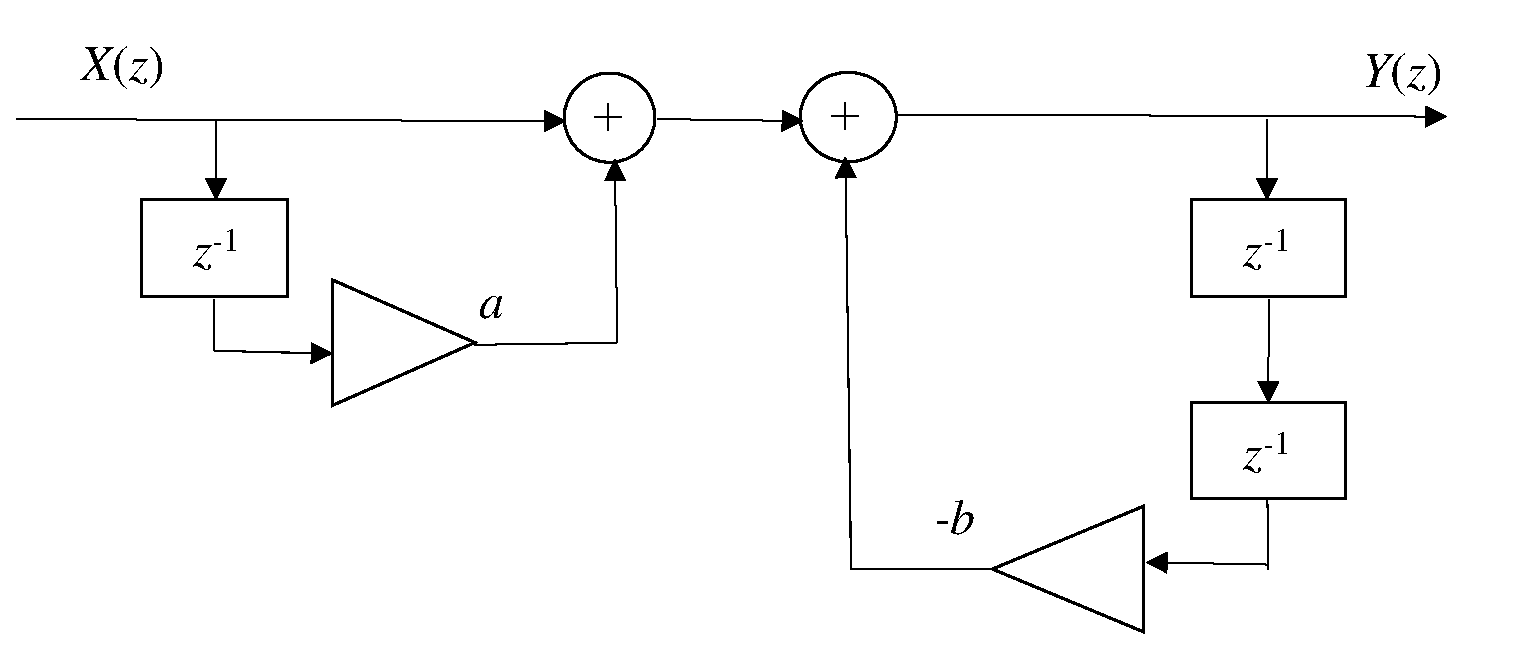
\includegraphics[width=.6\textwidth]{fig/zu-9e-1b.eps}
\end{center}
%\caption{システムのハードウェア構成}
%\label{fig:f-9e-a2}
%\end{figure}

\begin{displaymath}
(3) \hspace{3mm} Y(z)=X(z)+aY(z)z^{-1}+bY(z)z^{-2}=X(z)+(az^{-1}+bz^{-2})Y(z) \nonumber
\end{displaymath}
と書けることから,伝達関数$H(z)$は
\begin{displaymath}
H(z)=\frac{Y(z)}{X(z)}=\frac{1}{1-az^{-1}-bz^{-2}} \nonumber
\end{displaymath}
であるため,ハードウェア構成は下図のようになる.

%\begin{figure}[H]
\begin{center}
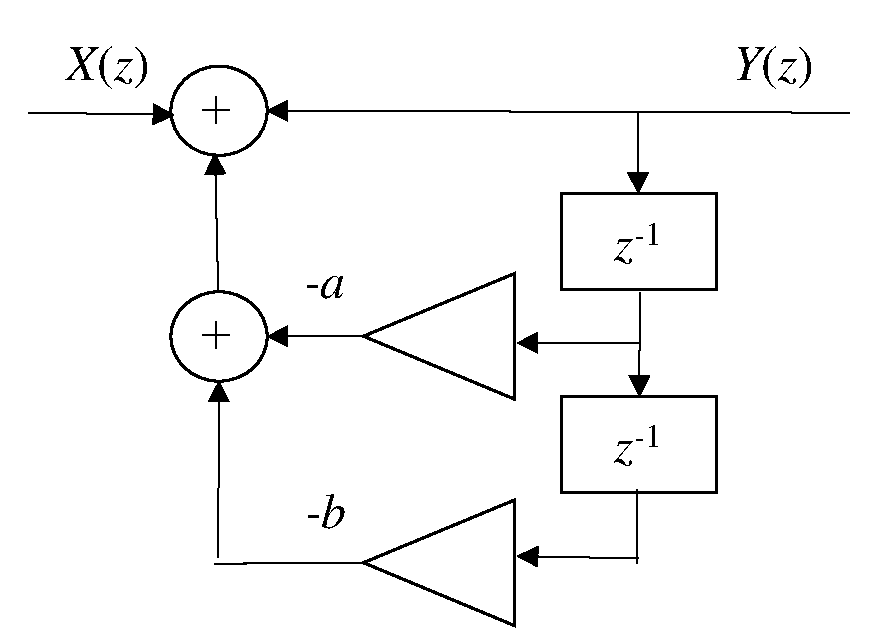
\includegraphics[width=.5\textwidth]{fig/zu-9e-1c.eps}
\end{center}
%\caption{システムのハードウェア構成}
%\label{fig:f-9e-a3}
%\end{figure}

\subsubsection*{問題\ref{chapter:42}.3}

\noindent (1) まず周波数特性について,$z$として$e^{j\omega }$を代入すると,
\begin{displaymath}
H(e^{j\omega }) = (1+2e^{-j\omega }+e^{-2j\omega }) = 2e^{-j\omega}(1+\cos(\omega)) \nonumber
\end{displaymath}
と書けるので
\begin{displaymath}
A(e^{j\omega }) = 2(1+\cos(\omega)) \nonumber
\end{displaymath}
\begin{displaymath}
\theta(e^{j\omega }) = -\omega \nonumber
\end{displaymath}
である.

この伝達関数は,
\begin{displaymath}
H(z)=1+2z^{-1}+z^{-2}=(1+z^{-1})^2=\frac{(1+z)^2}{z^2} \nonumber
\end{displaymath}
と書けることから,極は0の重根であり,安定なシステムである.

\noindent (2) まず伝達関数は
\begin{displaymath}
H(z)=\displaystyle \frac{1+2z^{-1}}{2+z^{-1}}=\displaystyle \frac{1+2z^{-1}}{z^{-1}(1+2z)} \nonumber
\end{displaymath}

周波数特性について,$z$として$e^{j\omega }$を代入すると,
\begin{displaymath}
H(e^{j\omega }) = \displaystyle \frac{1+2e^{-j\omega }}{e^{-j\omega }(1+2e^{j\omega })} \nonumber
\end{displaymath}
と書けるので
\begin{displaymath}
A(e^{j\omega }) = \frac{\sqrt{(1+2\cos(\omega))^2+(2\sin(\omega))^2}}{|e^{-j\omega }|\sqrt{(1+2\cos(\omega))^2+(2\sin(\omega))^2}}=1 \nonumber
\end{displaymath}
\begin{eqnarray}
\theta(e^{j\omega }) &=& \tan^{-1}\frac{2\sin(\omega)}{1+2\cos(\omega)}-\tan^{-1}\frac{-2\sin(\omega)}{1+2\cos(\omega)}+\omega \nonumber \\
&=& 2\tan^{-1}\frac{2\sin(\omega)}{1+2\cos(\omega)}+\omega \nonumber
\end{eqnarray}
である.

この伝達関数から,極は$1/2$であり,安定なシステムである.


\subsection*{第\ref{chapter:6}章}

\subsubsection*{問題\ref{chapter:6}.1}
\vskip-\baselineskip
\begin{displaymath}
(1) \hspace{3mm} X(\omega ) = \displaystyle \sum_{n=-^\infty }^{\infty }x(nT)e^{-j \omega nT}= \sum_{n=-^\infty }^{\infty }\delta (nT)e^{-j \omega nT} =1 \nonumber
\end{displaymath}

\begin{eqnarray}
(2) \hspace{3mm} X(\omega ) &=& \displaystyle \sum_{n=-^\infty }^{\infty } \left \{ u(nT)-u(nT-NT) \right \} 
= \sum_{n=0}^{N-1}e^{-j \omega nT} = \frac{1-e^{-jm\omega NT}}{1-e^{-j\omega T}} \nonumber \\
 &=& \frac{\sin 2\omega }{\sin \displaystyle \frac{\omega }{2}} 
\exp \left ( \displaystyle -j \frac{\omega T-j(N-1)}{2} \right ) \nonumber
\end{eqnarray}

\subsubsection*{問題\ref{chapter:6}.2}

\begin{displaymath}
\textrm{(a)} \hspace{3mm} X(j\omega ) = \left ( \displaystyle \frac{\sin \displaystyle \frac{2\omega t}{3}}{\sin \displaystyle \frac{\omega t}{3}} \right ) ^2
\end{displaymath}

\begin{displaymath}
\textrm{(b)} \hspace{3mm} X(j\omega ) = \left ( \displaystyle \frac{\sin \displaystyle \frac{2\omega t}{3}}{\sin \displaystyle \frac{\omega t}{3}} \right ) ^2 e^{-j2\omega t}
\end{displaymath}

\begin{eqnarray}
\textrm{(c)} \hspace{3mm} X(j\omega ) = \left ( \displaystyle \frac{\sin 3\omega t}{\sin \omega t} \right ) ^2 e^{-j4\omega t} \nonumber
\end{eqnarray}

\subsubsection*{問題\ref{chapter:6}.3}

$f_s>3$kHz


\subsection*{第\ref{chapter:a-filter}章}

\subsubsection*{問題\ref{chapter:a-filter}.1}

$-6$dB (常用対数表から$\log_{10}2 \fallingdotseq 0.301$なので$\log_{10}2$を0.3とみなしている)

\subsubsection*{問題\ref{chapter:a-filter}.2}

$C=\displaystyle \frac{1}{2\pi f R} \fallingdotseq 1.6 \times 10^{-6}$Fとなるので1.6$\mu$Fである.

\subsubsection*{問題\ref{chapter:a-filter}.3}

$C=\displaystyle \frac{1}{4\pi^2 f^2 L} \fallingdotseq 2.53 \times 10^{-12}$Fとなるので2.53pFである.


\subsubsection*{問題\ref{chapter:a-filter}.4}\vskip-.2\baselineskip
\begin{displaymath}
I=\displaystyle \left( \frac{V}{R}+ \frac{R}{j\omega L} +j\omega C \right )V \nonumber
\end{displaymath}


\subsection*{第\ref{chapter:dft}章}

\subsubsection*{問題\ref{chapter:dft}.1}

\begin{eqnarray}
\left( 
\begin{array}{cccc}
W^0 & W^0 & W^0 & W^0 \\
W^1 & W^2 & W^3 & W^4 \\
W^2 & W^4 & W^6 & W^8 \\
W^3 & W^6 & W^9 & W^12
\end{array}
\right)
\left( 
\begin{array}{c}
x[0] \\
x[1] \\
x[2] \\
x[3]
\end{array}
\right) = 
\left( 
\begin{array}{cccc}
1 & 1 & 1 & 1 \\
W^1 & W^2 & W^3 & W^4 \\
W^2 & W^4 & W^6 & W^8 \\
W^3 & W^6 & W^9 & W^{12}
\end{array}
\right)
\left( 
\begin{array}{c}
1 \\
1 \\
0 \\
1
\end{array}
\right) = 
\left( 
\begin{array}{c}
3 \\
1 \\
-1 \\
1
\end{array}
\right) \nonumber
\end{eqnarray}

\subsubsection*{問題\ref{chapter:dft}.2}

\begin{eqnarray}
X(k)=\left \{ 
\begin{array}{cc}
-jN/2 & (k=3) \\
jN/2 & (k=N-3) \\
0 & (それ以外)
\end{array}
\right . \nonumber
\end{eqnarray}


\subsection*{第\ref{chapter:fft}章}

\subsubsection*{問題\ref{chapter:fft}.1}

下図のようになる.

%\begin{figure}[H]
\begin{center}
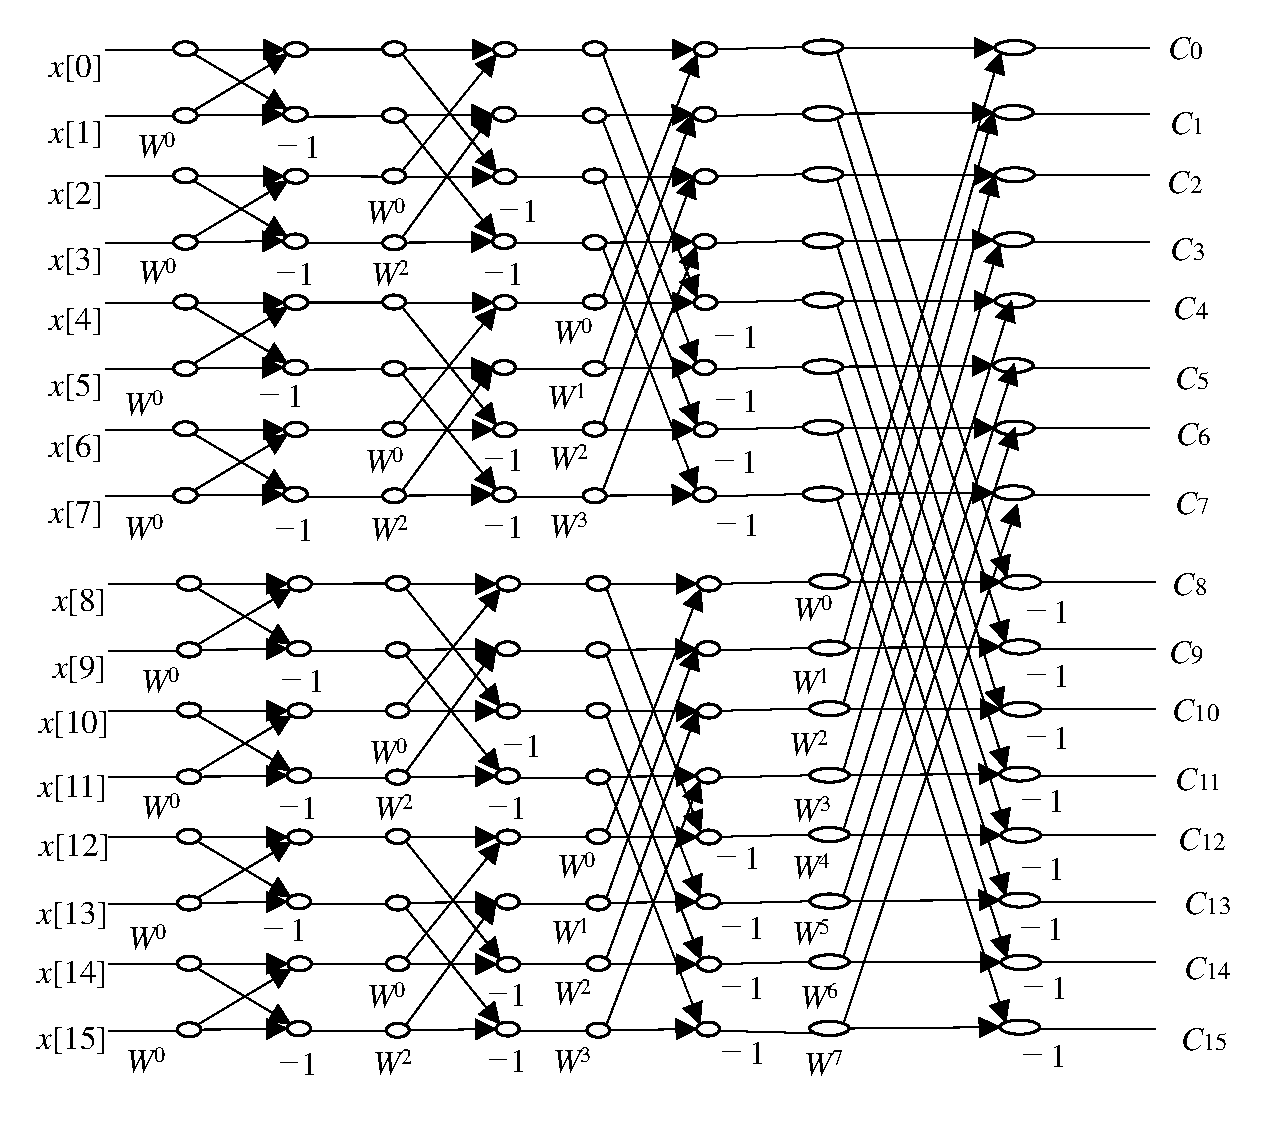
\includegraphics[width=.5\textwidth]{fig/zu-11e-1.eps}
\end{center}
%\caption{問題\ref{chapter:fft}.1の解図}
%\label{fig:zu-12e-01}
%\end{figure}


\subsection*{第\ref{chapter:window}章}

\subsubsection*{問題\ref{chapter:window}.1}

下図(b),(c)を得る.窓長が短いと,メインローブが近接スペクトルを含んでしまい,スペクトルの分離ができないことがわかる.また,サイドローブが大きいと,小さな値のスペクトルを検知することができない.

%\begin{figure}[H]
\begin{center}
\begin{minipage}{.35\textwidth}
\begin{center}
%\includegraphics[width=8cm]{fig/fig-5-14.eps}
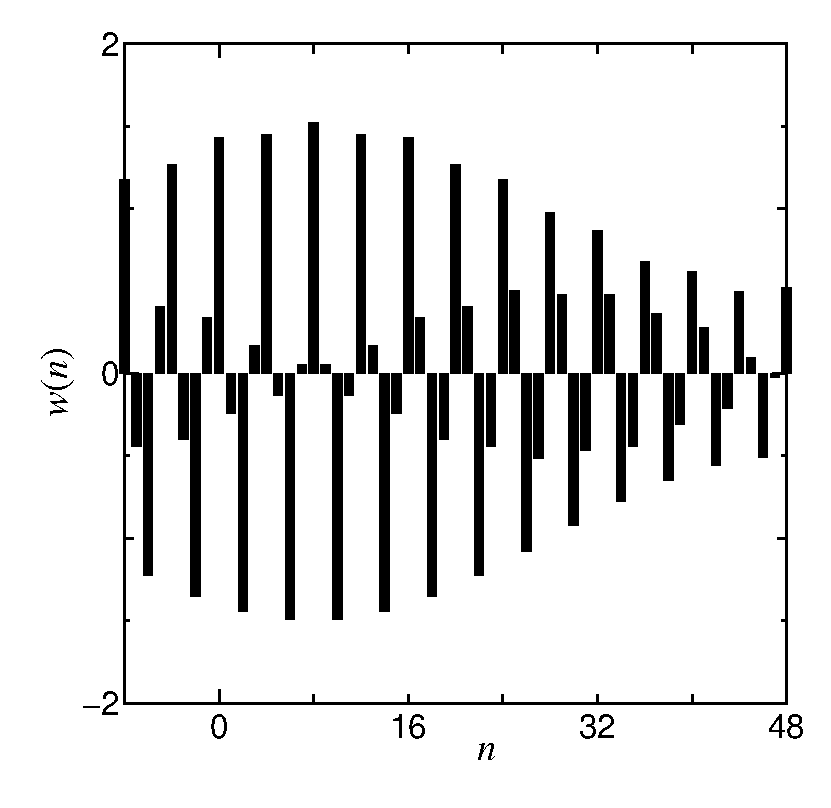
\includegraphics[width=.98\textwidth]{fig/zu-5-14-a.eps}

(a) 信号波形
\end{center}
\end{minipage}
\begin{minipage}{.35\textwidth}
\begin{center}
%\includegraphics[width=8cm]{fig/fig-5-14.eps}
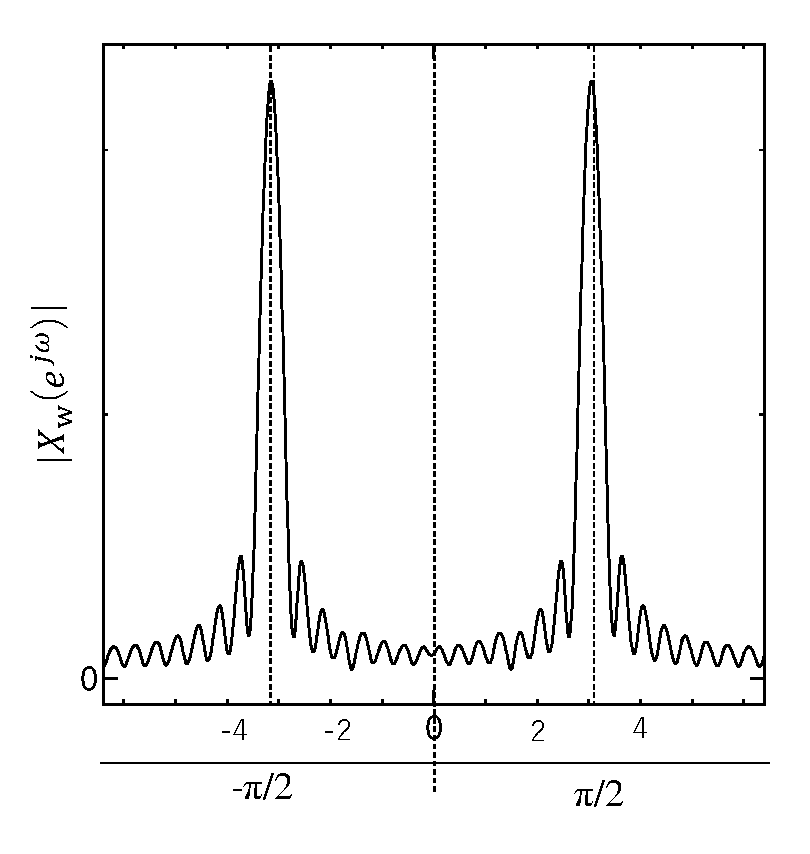
\includegraphics[width=.98\textwidth]{fig/zu-5-14-b.eps}

(b) $M=32$のときのスペクトル
\end{center}
\end{minipage}\\[.5\baselineskip]
\begin{minipage}{.35\textwidth}
\begin{center}
%\includegraphics[width=8cm]{fig/fig-5-14.eps}
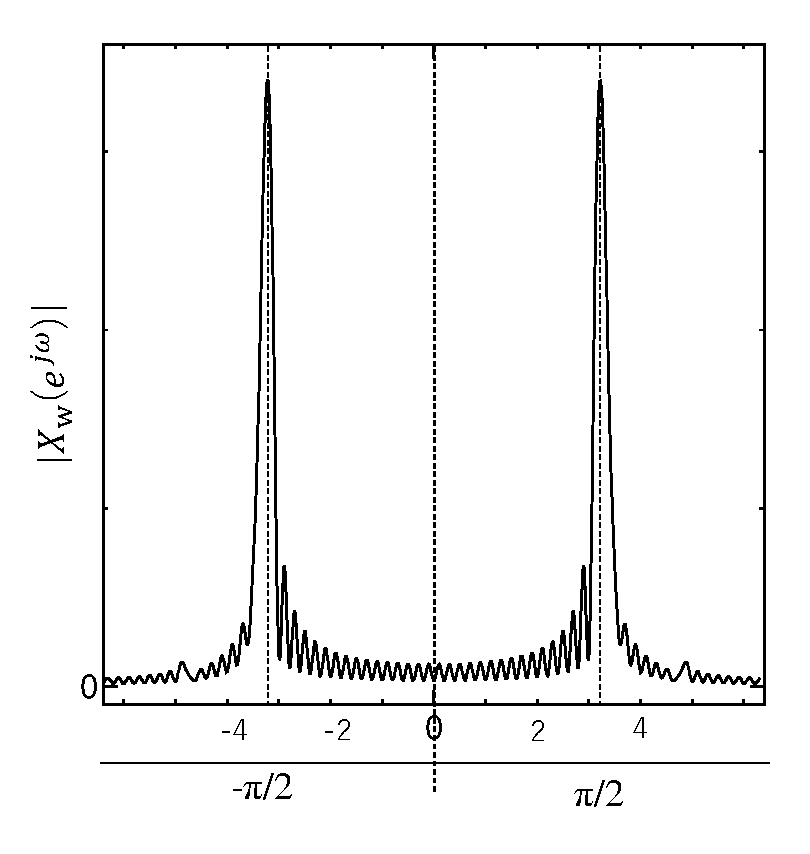
\includegraphics[width=.98\textwidth]{fig/zu-5-14-c.eps}

(c)  $M=64$のときのスペクトル
\end{center}
\end{minipage}
\end{center}
%\caption{例題5.4}
%\label{fig:5-14}
%\end{figure}


\subsection*{第\ref{chapter:11}章}

\subsubsection*{問題\ref{chapter:11}.1}

下図のようになる.

%\begin{figure}[H]
\begin{center}
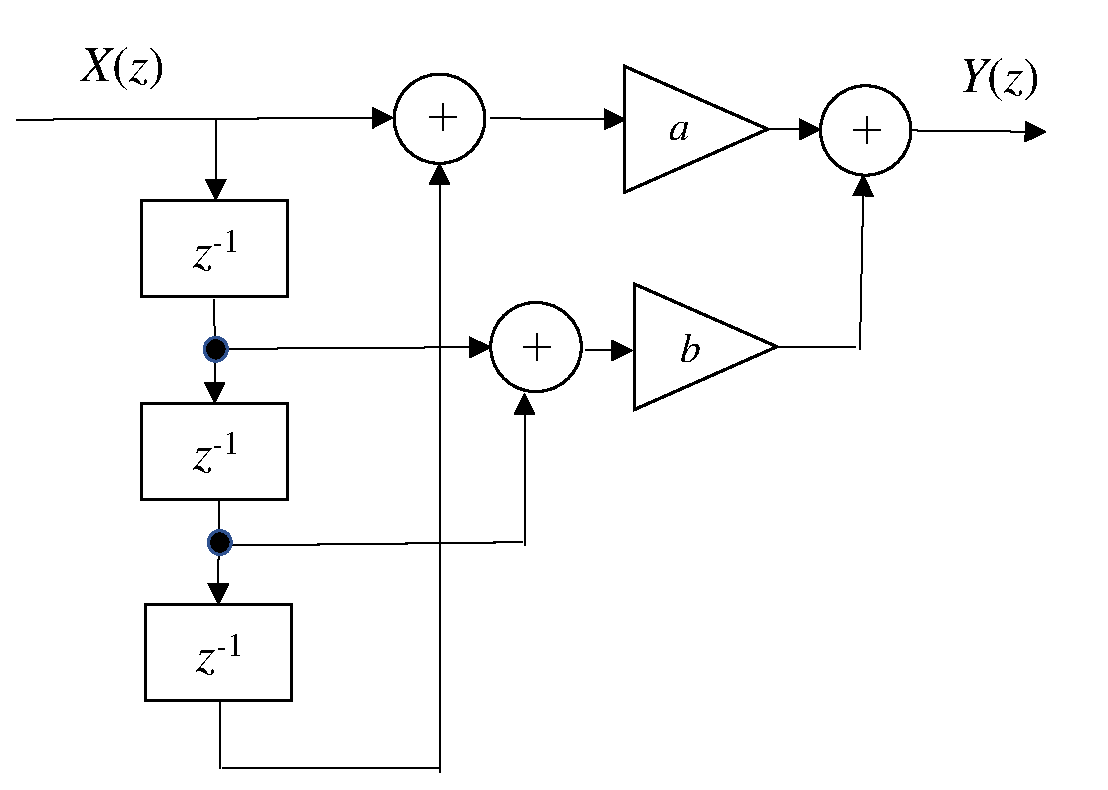
\includegraphics[width=.6\textwidth]{fig/zu-12e-1.eps}
\end{center}
%\caption{問題\ref{chapter:11}.1の解図}
%\label{fig:zu-12e-1}
%\end{figure}



\subsection*{第\ref{chapter:image}章}

\subsubsection*{問題\ref{chapter:image}.1}

下図のようになる.
%\begin{figure}[h]
\begin{center}
\begin{minipage}{7cm}
\begin{center}
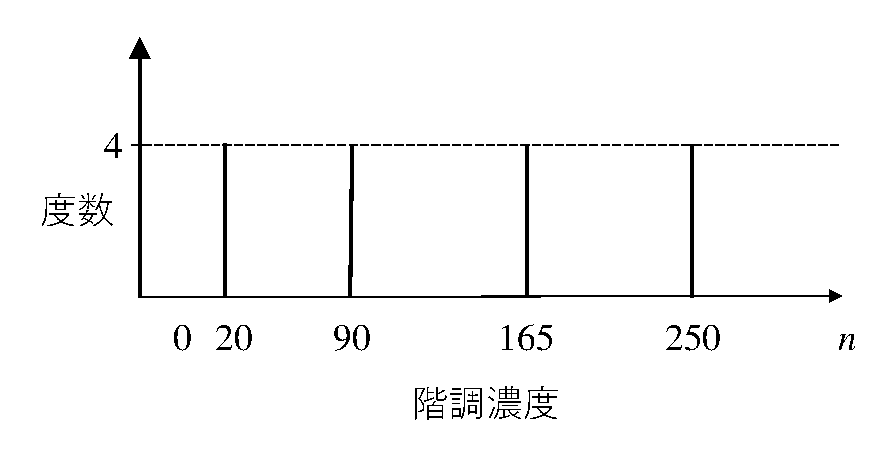
\includegraphics[width=6.5cm]{fig/image_hist.eps}

(1) ヒストグラム
\end{center}
\end{minipage}\\[.5\baselineskip]
\begin{minipage}{.3\textwidth}
\begin{center}
\begin{tabular}{|c|c|c|c|}
\hline
235 & 165 & 90 & 5 \\
\hline 
235 & 165 & 90 & 5 \\
\hline
235 & 165 & 90 & 5 \\
\hline
235 & 165 & 90 & 5 \\
\hline 
\end{tabular}

(2)ネガポジ画像
\end{center}
\end{minipage}\\[.5\baselineskip]
\begin{minipage}[t]{.3\textwidth}
\begin{center}
\begin{tabular}{|c|c|c|c|}
\hline
255 & 0 & 255 & 255 \\
\hline 
0 & 255 & 0 & 255 \\
\hline
0 & 0 & 255 & 255 \\
\hline
0 & 0 & 0 & 255 \\
\hline 
\end{tabular}

(3) ディザ法による2値画像
\end{center}
\end{minipage}\ \ 
\begin{minipage}[t]{.5\textwidth}
\begin{center}
\begin{tabular}{|c|c|c|c|}
\hline
%0 & 8 & 2 & 10 \\
8 & 136 & 40 & 168 \\
\hline 
200 & 72 & 232 & 104 \\
\hline
56 & 184 & 24 & 152 \\
\hline
248 & 120 & 216 & 88 \\
\hline 
\end{tabular}

(3') ディザ法における閾値(図\ref{fig:dither_m}の値に16を掛けて8を足している)
\end{center}
\end{minipage}

%\caption{問題\ref{chapter:image}.1の解図}
%\label{fig:zu-13-1a}
\end{center}
%\end{figure}




